\documentclass[11pt]{article}

\usepackage{epsfig}
\usepackage{graphics}
\usepackage{graphicx}
%\usepackage[german]{babel}
\usepackage{german}
\usepackage[utf8]{inputenc}       %% deutsche Umlaute wie normale
                             %% Buchstaben verwenden
                             %% (ansonsten muesste durch "a getippt werden)
\usepackage{url}
\newcommand{\urlBiBTeX}[1]{\url{#1}}
% Seiten-Layout
% Mit diesen Kommandos werde die R�der auf dem Papier
% festgelegt. Dies wurde 1:1 bernommen.

\setlength{\textwidth}{6.5in}            % Textbreite
\setlength{\hoffset}{0in}
\setlength{\voffset}{0in}
%\setlength{\evensidemargin}{-.0in}
\setlength{\textheight}{9in}          % Texth�e 
\setlength{\topmargin}{-0.2in}           % oberer Rand
\setlength{\oddsidemargin}{+.1cm}     % linker Rand
%\setlength{\marginparwidth}{-0.6cm}    % rechter Rand

\setlength\parskip{\medskipamount}
\setlength\parindent{0pt}
\thispagestyle{empty}
\begin{document}
\begin{center}
\scalebox{0.9}{
\includegraphics{header_hwr.eps}}
\end{center}

\vspace{0.6cm}
\begin{center}
\begin{LARGE}Seminar \\ \end{LARGE}
\vspace{0.2cm}
\begin{LARGE}Aktuelle Themen des Hardwareentwurfs \\ \end{LARGE}
\vspace{2.9cm}
\begin{LARGE}\textbf{Dein Thema }\\ \end{LARGE}
\vspace{2.9cm}
\begin{LARGE}Dein Name \\ \end{LARGE}
\vspace{10.2cm}
\begin{large}Sommersemester 2008\\ \end{large}


\end{center}
\vspace{0.4cm}\ \\
\newpage
\tableofcontents
\newpage

\section{Einleitung}
Hier ist die Einleitung, es wird z.B. so eine Literaturangabe eingebunden \cite{halbleiter}. Die Abbildung \ref{pic_einfuehrung} ist als Beispiel eingebunden, wie man ein Bild in das Dokument einfügt.
\begin{figure}[htb]
	\begin{center}
	\scalebox{0.8}{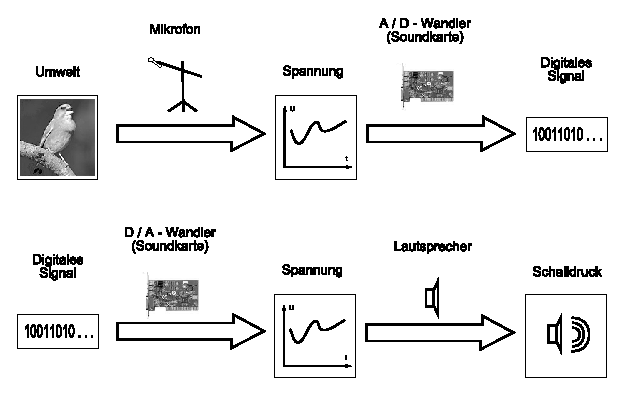
\includegraphics{Einfuehrung.eps}}
		\caption{Schnittstelle "`Digitales System / Umwelt"'}
	\label{pic_einfuehrung}
	\end{center}
\end{figure}

\section{Zusammenfassung}


\bibliographystyle{unsrt}


\bibliography{seminar}
\end{document}
